% =====================================================================
% NeurIPS workshop submission.
% Drop the workshop's official style file (e.g. neurips_2026.sty) next to
% this file. Compiles with pdflatex + bibtex.
% All families are evaluated OUT-OF-SAMPLE on the same shared held-out
% trajectories (movement_id); references.bib verified against arXiv (June 2026).
% =====================================================================
\documentclass{article}

% --- NeurIPS 2026 style. Currently set to PREPRINT (authors shown, with a
%     "Preprint. Work in progress." footer). To switch:
%       * anonymous submission  -> \usepackage{neurips_2026}            (adds line numbers, anonymizes)
%       * workshop submission    -> \usepackage[sglblindworkshop]{neurips_2026}  (single-blind)
%                                or \usepackage[dblblindworkshop]{neurips_2026}  (double-blind)
%                                   AND set \workshoptitle{...} below
%       * camera-ready           -> add the "final" option, e.g. [sglblindworkshop, final]
% -------------------------------------------------------------------------------
\IfFileExists{neurips_2026.sty}{%
  \usepackage[preprint]{neurips_2026}%
}{%
  \usepackage[margin=1in]{geometry}\usepackage{parskip}\usepackage{natbib}%
}

\usepackage[utf8]{inputenc}
\usepackage[T1]{fontenc}
\usepackage{hyperref}
\usepackage{url}
\usepackage{booktabs}
\usepackage{amsfonts,amsmath,amssymb}
\usepackage{microtype}
\usepackage{graphicx}
\usepackage{pgfplots}
\pgfplotsset{compat=1.18}
\usepackage{xcolor}
\usepackage{siunitx}
\usepackage{multirow}
\usepackage{enumitem}

\title{Forecasting Chaos Across Model Families: An Out-of-Sample,
Reliability-Adjusted Benchmark}
% Required when using a workshop option (sgl/dblblindworkshop):
% \workshoptitle{Name of the NeurIPS 2026 Workshop}

\author{%
  Sriman Narayan Kandi\thanks{Corresponding author.} \\
  Independent Researcher \\
  \texttt{kandisriman@gmail.com} \\
  \And
  Trishant Srinivasan \\
  Independent Researcher \\
}

\begin{document}
\maketitle

\begin{abstract}
This paper evaluates chaotic forecasting across model families under a shared
out-of-sample protocol. The benchmark is a controlled $k$-pendulum system
($k\in\{1,2,3\}$; chaotic for $k\ge2$) with four families: large language models
(LLMs), Chronos, learned dynamics models (Neural~ODE, HNN, LNN), and classical
integrators. Reliability-adjusted scoring assigns a fixed error to refusals and
parse failures rather than discarding them. Off their training trajectories,
learned dynamics models increase from $\sim$0.26 to 0.97--1.14\,rad for the
stable variants and do not outperform the linearized-dynamics or nearest-neighbor
baselines. Among the evaluated black-box methods, \texttt{kimi} has the lowest
error ($0.538$\,rad), while known-physics integrators remain the numerical
reference. Objective effects are architecture-dependent: mixed-$k$ rollout is
lower for the Neural~ODE, whereas single-$k$ rollout is lower for the HNN. A
matched disclosure experiment and inference probe find little evidence that the
LLMs infer hidden physical constants; under this protocol they default to
Earth-standard values. Cost is also asymmetric: the LLM run is the only
per-query billed evaluation. The results indicate that in-sample evaluation can
overestimate learned-dynamics performance and motivate controlled out-of-sample
comparison of scientific forecasting methods.
\end{abstract}

\section{Introduction}
Comparing forecasting methods on a chaotic system depends on evaluation design: whether
models are scored in or out of sample, how failures are handled, and what information each
model receives. We evaluate LLMs, time-series foundation models, learned dynamics models,
and classical integrators on a shared $k$-link pendulum benchmark. Given state
$\mathbf{s}_t$, the task is to predict $\mathbf{s}_{t+T}$. The pendulum is integrable at
$k{=}1$ and chaotic for $k{\ge}2$, has high-precision ground truth, and requires no
domain-specific grading.

\paragraph{Contributions.}
\begin{enumerate}[leftmargin=1.4em,itemsep=2pt,topsep=2pt]
\item A \textbf{cross-family evaluation protocol} in which all families are scored on the
same out-of-sample held-out trajectories, with a reliability-adjusted metric that assigns a
fixed error to abstentions rather than discarding them
(\S\ref{sec:metrics}, \S\ref{sec:reliability}).
\item An \textbf{out-of-sample leaderboard}: tested off their training trajectories the
learned models reach 0.97--1.14\,rad for the stable variants (from $\sim$0.26 in-sample) and
do not outperform the linearized-dynamics or nearest-neighbor baselines,
while among the evaluated black-box methods the lowest error is obtained by \texttt{kimi}
(0.538\,rad). Objective effects are architecture-dependent rather than uniformly favorable to
one training loss (\S\ref{sec:objective}).
\item \textbf{Chaos-appropriate analysis}: a predictability-horizon metric and a
confound-free system-identification test. An unadjusted regime contrast suggests lower
error when constants are hidden; a matched paired experiment and a direct inference probe
indicate that this is a difficulty confound rather than parameter inference
(\S\ref{sec:sysid}).
\end{enumerate}

\section{Related Work}
\paragraph{Learned dynamics.} Neural~ODEs learn a continuous-time vector field from
data~\citep{chen2018node}. Hamiltonian Neural Networks impose an energy-conserving inductive
bias through a learned Hamiltonian~\citep{greydanus2019hnn}; Lagrangian Neural Networks
enforce the Euler--Lagrange equations through second-order autodifferentiation
\citep{cranmer2020lnn}. Chaotic systems such as the Lorenz attractor and the double pendulum
are standard testbeds~\citep{gilpin2021chaos}. We evaluate all three against general-purpose
models under matched conditions.

\paragraph{Foundation models as forecasters.} LLMs can act as zero-shot time-series
forecasters when series are serialized as text~\citep{gruver2023llmtime}, and time-series
foundation models---Chronos~\citep{ansari2024chronos}, TimesFM~\citep{das2024timesfm}, and
Moirai~\citep{woo2024moirai}---are trained for general forecasting.
\citet{zhang2025zeroshotchaos} study zero-shot forecasting of chaotic systems with such
models. We evaluate these forecasters on the same grid as physics-informed and language models.

\paragraph{LLMs for physical and mathematical reasoning.} LLMs perform well on mathematical
problem solving~\citep{lewkowycz2022minerva} and, with chain-of-thought prompting, on
multi-step reasoning~\citep{wei2022cot}; recent benchmarks probe physics reasoning in LLMs
\citep{xu2025ugphysics}. Our task instead requires quantitative trajectory prediction of a
chaotic system rather than qualitative or symbolic reasoning.

\section{Benchmark Design}
\paragraph{Choice of system.} We use the $k$-link pendulum to study evaluation methodology,
not pendulums as an application domain. It provides a tunable chaos axis, high-precision
ground truth, known equations for numerical references, and controllable constants for the
system-identification test (\S\ref{sec:sysid}). The single controlled system is therefore a
deliberate design choice.

\subsection{Task and systems}
Given the state $\mathbf{s}_0=(\theta_1,\dots,\theta_k,\omega_1,\dots,\omega_k)\in
\mathbb{R}^{2k}$ of a $k$-link pendulum at $t{=}0$, the task is to predict $\mathbf{s}_T$ at
horizon $T$. Ground-truth trajectories integrate the full nonlinear Lagrangian equations of
motion with fixed-step RK4 at $\Delta t{=}10^{-3}$\,s, recording states every $0.01$\,s plus
a $10$\,s pre-$t{=}0$ context window (used only by the time-series models). Initial
conditions are sampled $\theta_i\sim\mathcal{U}(-3,3)$\,rad,
$\omega_i\sim\mathcal{U}(-1,1)$\,rad/s with a fixed seed. Because the labels are produced by
RK4 at this step, the RK4 baseline reported later (the same integrator at a $10{\times}$
coarser $\Delta t{=}10^{-2}$) is a numerical reference by construction rather than an independent
competitor; Euler and the symplectic integrator are distinct known-physics methods. Inputs
available to each family are stated in \S\ref{sec:inputs}.

\subsection{Regimes and grid}
Three regimes test generalization to non-standard constants (Table~\ref{tab:regimes}). In
\texttt{changed\_hidden} the constants $(g,L,m,\text{damping})$ are not disclosed to the
model, which makes the cell an in-context system-identification problem. An evaluation cell
is a tuple (model, $k$, regime, modality, horizon, prompting); horizons are
$\{0.01,1,10,60\}$\,s, modalities $\{$coords, image, image+coords$\}$ (LLMs only), and
prompting $\{$direct, chain-of-thought$\}$ (LLMs only). Non-LLM models use the
coordinate/direct setting.

\paragraph{Out-of-sample protocol.} Learned dynamics models are evaluated off their training
data. We generate a shared held-out set (a separate seed from the training trajectories) of
$180$ initial conditions ($60$ per regime, spanning $k\in\{1,2,3\}$) and evaluate every
family on the identical trajectories, keyed by \texttt{movement\_id}. The cross-family
leaderboard (\S\ref{sec:reliability}) uses horizons $\{1,10\}$\,s, where chaos has begun but
error has not saturated (\S\ref{sec:metrics}), giving $180\times2=360$ cells per model. We
report no in-sample numbers and quantify the size of the in-sample effect directly
(\S\ref{sec:reliability}).

\begin{table}[tbp]
\centering\small
\caption{Physical regimes. \texttt{changed\_hidden} withholds the constants.}
\label{tab:regimes}
\begin{tabular}{lccccc}
\toprule
Regime & $g$ (m/s$^2$) & $L$ (m) & $m$ (kg) & damping & disclosed \\
\midrule
\texttt{normal} & 9.81 & 1.0 & 1.0 & 0.0 & --- \\
\texttt{changed\_disclosed} & 3.71 & 1.4/0.7/1.1 & 2.0/0.6/1.5 & 0.05 & yes \\
\texttt{changed\_hidden} & 1.62 & 0.8/1.2/0.9 & 0.5/1.8/1.0 & 0.10 & no \\
\bottomrule
\end{tabular}
\end{table}

\subsection{Inputs and grouping}
\label{sec:inputs}
Table~\ref{tab:inputs} states what each family receives. Chronos is a time-series model, so
we evaluate it in its standard form: a history-conditioned forecaster with a $10$\,s
pre-$t{=}0$ context window. The LLMs and learned dynamics models are state-conditioned from
$t{=}0$. For learned models, hidden-regime cells are equalized by withholding hidden constants
and using normal-regime prior constants. A separate asymmetry runs in the opposite direction:
the LLMs are large-scale proprietary models, whereas the learned models are small
($256$-wide, $3$-layer MLPs trained on a single $8$\,GB GPU; Appendix~B). The behavior of
larger physics-informed networks is outside the scope of this study. We separate
known-physics methods (RK4, Euler, symplectic) from black-box methods (LLMs, Chronos,
learned dynamics); the former are numerical references.

\begin{table}[tbp]
\centering\small
\caption{Inputs available to each family. State is at $t{=}0$; history is pre-$t{=}0$.
Chronos is history-conditioned; learned \texttt{hidden} cells withhold hidden constants.}\label{tab:inputs}
\begin{tabular}{lcccc}
\toprule
Family & State & History & Constants & Equations \\
\midrule
Numerical (RK4/Euler/sympl.) & \checkmark & --- & \checkmark\ (all regimes) & \checkmark\ (exact) \\
Learned (NODE/HNN/LNN) & \checkmark & --- & \checkmark\ base; withheld$^\ast$ & --- (learned) \\
Time-series (Chronos) & --- & \checkmark\ ($10$\,s context) & --- & --- \\
LLMs (kimi/grok/deepseek) & \checkmark & --- & except \texttt{hidden} & --- \\
\bottomrule
\end{tabular}
\end{table}

\subsection{Metrics}
\label{sec:metrics}
The primary error is the mean absolute angle error (radians), wrapped to $[-\pi,\pi]$ and
averaged over links and trajectories; we also track Cartesian bob error, angular-velocity
sign match, and energy drift. Three choices are specific to this setting.

\paragraph{Reliability-adjusted error.} A cell is answered only if the model returns a
parseable, finite prediction. Reporting error over answered cells alone would reward
abstention on hard cells. We therefore assign unanswered cells the random-guess baseline
$\pi/2$ (the expected wrapped-angle error of a uniform guess); we also report the strict
upper bound $\pi$. Answering is thus part of the score.

\paragraph{Predictability horizon.} For chaotic systems, pointwise error past the Lyapunov
time saturates to a system-dependent constant for every model, so long-horizon error
rankings carry little information. We define the predictability horizon as the longest
horizon a model tracks contiguously below a threshold $\tau$, starting from $t{=}0$: we walk
horizons in increasing order and stop at the first that exceeds $\tau$. The contiguous rule
is used because, after divergence, a later horizon can fall below $\tau$ by angle-wrap
coincidence. We sweep $\tau$.

\paragraph{System-identification gap.} We define
$\Delta_{\mathrm{sysid}}=\mathrm{err}(\text{hidden})-\mathrm{err}(\text{disclosed})$.
Positive values indicate a penalty for withholding constants. Because regime contrasts
confound disclosure with trajectory difficulty, we also run a matched experiment
(\S\ref{sec:sysid}) that toggles disclosure on identical trajectories and asks hidden-condition
models to report inferred constants.

\section{Methods}
\label{sec:methods}
\paragraph{LLMs.} We evaluate \texttt{kimi-k2.6}, \texttt{grok-4-1-fast-reasoning}, and
\texttt{deepseek-v4-pro} through an OpenAI-compatible API (Azure AI Foundry deployments;
evaluated June~2026), with a structured prompt (system description, disclosed constants where
applicable, initial state) and a JSON answer schema (Appendix~A). Each cell uses one
temperature-$0$ call with a uniform token and timeout budget; no best-of-$N$ aggregation is
used. The LLM evaluation (Parts~A and~B, $3{,}960$ cells) records prompt and completion
token counts and has an estimated nominal API cost of \$110.38 under the pricing assumptions
in the released analysis script.

\paragraph{Time-series foundation models.} We run Chronos~\citep{ansari2024chronos} locally
on a single GPU in its standard history-conditioned form: the $10$\,s pre-$t{=}0$ context
window of all $2k$ state channels, resampled to up to $512$ points, forecasts to the target
horizon (prediction length $\le 64$ steps). The leaderboard uses \texttt{chronos-2} in
univariate and multivariate modes; the latter forecasts all $2k$ channels jointly. The
paired mode comparison uses $20$ trajectories per (k, regime) cell. The earlier
\texttt{chronos-t5-large} was preliminary; Moirai's \texttt{uni2ts} could not be installed
in our environment.

\paragraph{Learned dynamics.} Neural~ODE, HNN, and LNN share a $256$-wide, $3$-layer tanh
MLP and integrate at inference with \texttt{scipy}. We compare two objectives: derivative
matching (MSE on finite-difference $\dot{\mathbf{s}}$) and rollout loss (MSE on the state
after $k$ Euler steps, with gradients through the unroll). We also use mixed-$k$ rollout,
which trains on several window lengths jointly (Neural~ODE: $k\in\{10,50\}$; HNN:
$k\in\{5,20\}$). The LNN's loss requires second-order autodifferentiation, which Apple's MPS
backend does not run; we train it at full scale ($67$k samples, hidden 256) on a CUDA GPU.
All learned models are trained on the same nine trajectories---one per (k, regime) cell
(Appendix~B), a small budget for a chaotic system.

\paragraph{Integrators.} Euler, RK4, and St\"ormer--Verlet (symplectic) at $\Delta
t{=}0.01$\,s using the exact equations of motion; their error is from discretization alone.
RK4 is the data-generating process and serves as a numerical reference rather than an independent
competitor.

\paragraph{Baselines.} Four reference baselines use the same grid: persistence
($\theta_T{=}\theta_0$), constant velocity ($\theta_T{=}\theta_0{+}\omega_0T$), a
small-angle linearized model, and a nearest-neighbor analog forecast from the matching
(k, regime) training trajectory. The nearest-neighbor baseline uses the same data as the
learned models.

\section{Results}
\subsection{Out-of-sample leaderboard}
\label{sec:reliability}
Table~\ref{tab:overall} reports the out-of-sample leaderboard on the shared held-out set
($360$ cells: $180$ trajectories $\times$ horizons $\{1,10\}$\,s), using the
reliability-adjusted metric. Every model is scored on the same grid; the Answered column is
the fraction of valid predictions. LLMs use direct-prompt forecasts. Confidence intervals are
$95\%$ paired bootstrap over trajectories ($B{=}10^4$); for LLMs they do not include
per-call sampling variation.

The classical integrators have the lowest error: RK4 (the data-generating process) at
$0.059$, symplectic at $0.205$, Euler at $0.405$. Among the black-box
methods evaluated, the lowest error is obtained by \texttt{kimi} ($0.538$\,rad, $99\%$
answered), below both Chronos modes and all learned dynamics models. The four baselines
provide reference scores. \texttt{kimi} is below every baseline with a non-overlapping
confidence interval (the closest, nearest-neighbor, is $0.725$), so its standing is not an
explained by the scoring rule; both Chronos modes are also below the nearest-neighbor baseline in point
estimate. The learned dynamics models are not: after replacing the hidden-regime cells with
the equalized no-hidden-constants run, the nearest-neighbor analog lookup ($0.725$) and the
linearized-pendulum baseline ($0.855$) are below every learned model. Persistence ($1.004$)
is also below all learned models except HNN-rollout ($0.972$), with intervals overlapping for
the closest comparisons. Out of sample the learned models therefore do not outperform the
linearized or nearest-neighbor baselines, despite those baselines using the same training data. They score
$\sim$0.26\,rad under in-sample evaluation and reach $0.97$--$1.14$\,rad here for the stable
learned models; this factor of approximately four indicates that their in-sample strength on
this benchmark is largely attributable to evaluation on their training trajectories.

\begin{table}[tbp]
\centering\small
\caption{Out-of-sample leaderboard on the shared held-out set ($360$ cells, horizons
$\{1,10\}$\,s). Reliability-adjusted mean angle error (rad): unanswered or missing cells
scored at $\pi/2$; $95\%$ bootstrap CI. RK4 is the data-generating process and is reported
as a numerical reference. Methods new in this work are marked $\dagger$; simple baselines are
marked $\ddagger$.}\label{tab:overall}
\begin{tabular}{rlcccl}
\toprule
\# & Model & Err & 95\% CI & Answered & Family \\
\midrule
-- & rk4 (reference) & 0.059 & [0.032, 0.089] & 100\% & numerical \\
1 & symplectic & 0.205 & [0.163, 0.251] & 100\% & numerical \\
2 & euler & 0.405 & [0.344, 0.470] & 100\% & numerical \\
3 & kimi-k2.6 & 0.538 & [0.475, 0.602] & 99\% & LLM \\
4 & chronos2-multi$^\dagger$ & 0.684 & [0.617, 0.752] & 100\% & time-series \\
5 & chronos2-uni$^\dagger$ & 0.697 & [0.631, 0.766] & 100\% & time-series \\
6 & nearest-neighbor$^\ddagger$ & 0.725 & [0.657, 0.797] & 100\% & baseline \\
7 & linearized$^\ddagger$ & 0.855 & [0.774, 0.939] & 100\% & baseline \\
8 & grok-4-1-fast-reasoning & 0.881 & [0.805, 0.957] & 82\% & LLM \\
9 & deepseek-v4-pro & 0.952 & [0.881, 1.027] & 100\% & LLM \\
10 & hnn-rollout & 0.972 & [0.898, 1.047] & 100\% & learned \\
11 & persistence$^\ddagger$ & 1.004 & [0.934, 1.078] & 100\% & baseline \\
12 & neural-ode-rollout-mixed$^\dagger$ & 1.036 & [0.967, 1.104] & 100\% & learned \\
13 & hnn-rollout-mixed$^\dagger$ & 1.066 & [0.990, 1.143] & 100\% & learned \\
14 & neural-ode & 1.110 & [1.039, 1.181] & 100\% & learned \\
15 & neural-ode-rollout & 1.121 & [1.054, 1.190] & 100\% & learned \\
16 & hnn & 1.138 & [1.059, 1.218] & 100\% & learned \\
17 & constant-velocity$^\ddagger$ & 1.319 & [1.241, 1.396] & 100\% & baseline \\
18 & lnn$^\dagger$ (full-scale) & 1.349 & [1.283, 1.416] & 66\% & learned \\
\bottomrule
\end{tabular}
\end{table}

\paragraph{Effect of the reliability adjustment.} \texttt{grok} answers $82\%$ of the grid
and \texttt{lnn} $66\%$; scoring those abstentions at $\pi/2$, rather than averaging over
answered cells, places them below more reliable methods. Averaging over answered cells alone would
rank the least reliable models higher.

\subsection{Behavior by horizon}
\label{sec:behavior}
Out-of-sample error by horizon appears in Appendix~D (Table~\ref{tab:horizon}). At $1$\,s the ordering
follows the leaderboard: the integrators are near-exact, \texttt{kimi} ($0.457$) has the
lowest black-box error, and the learned models are at $0.86$--$1.26$. At $10$\,s all models
are in the chaotic regime, and the ordering is stable: \texttt{kimi} ($0.619$) remains lowest
among black-box methods while the learned models reach $1.09$--$1.44$. The mixed-$k$
Neural~ODE, which is the in-sample standout at $1$--$10$\,s, is mid-pack here ($0.951$ /
$1.120$). Figure~\ref{fig:errorgrowth} shows the growth curves over the
$\{0.01,1,10,60\}$\,s ladder: the numerical integrators stay near zero until ${\sim}10$\,s,
whereas every black-box family saturates near the chaotic noise floor by $1$\,s. The
$\{1,10\}$\,s window used for the leaderboard is the range over which the families remain
separable.

% (Table tab:horizon relocated to Appendix D)

\begin{figure}[tbp]
\centering
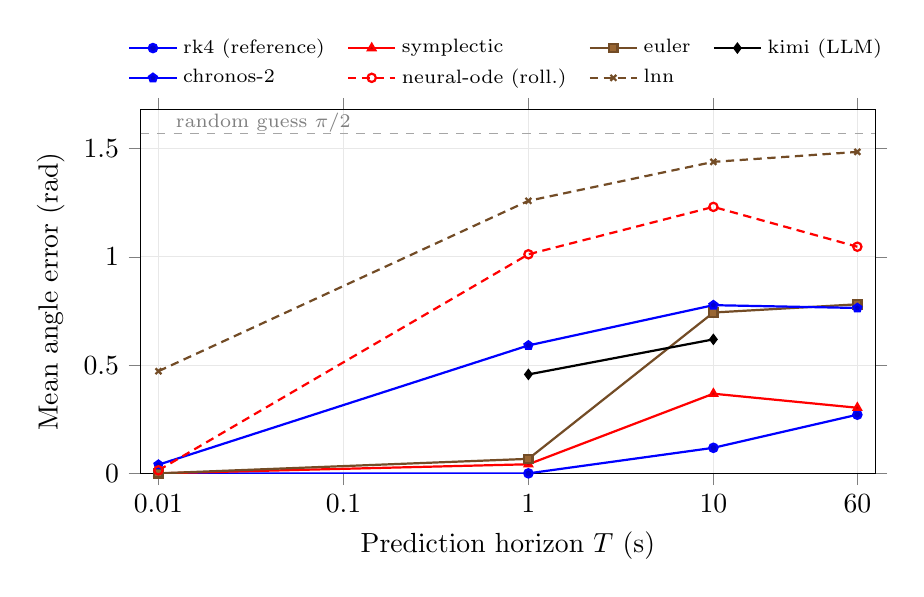
\begin{tikzpicture}
\begin{semilogxaxis}[
  width=0.9\linewidth, height=6.2cm,
  xlabel={Prediction horizon $T$ (s)}, ylabel={Mean angle error (rad)},
  xmin=0.008, xmax=75, ymin=0, ymax=1.68,
  xtick={0.01,0.1,1,10,60}, log ticks with fixed point,
  legend columns=4,
  legend style={at={(0.5,1.03)}, anchor=south, font=\scriptsize, draw=none, fill=none,
                cells={anchor=west}, /tikz/every even column/.append style={column sep=6pt}},
  grid=both, grid style={gray!18}, tick align=outside,
  every axis plot/.append style={thick, mark size=1.5pt},
]
\addplot+[mark=*]         coordinates {(0.01,0.000) (1,0.000) (10,0.118) (60,0.271)};
\addlegendentry{rk4 (reference)}
\addplot+[mark=triangle*] coordinates {(0.01,0.000) (1,0.042) (10,0.368) (60,0.303)};
\addlegendentry{symplectic}
\addplot+[mark=square*]   coordinates {(0.01,0.000) (1,0.067) (10,0.743) (60,0.781)};
\addlegendentry{euler}
\addplot+[mark=diamond*]  coordinates {(1,0.457) (10,0.619)};
\addlegendentry{kimi (LLM)}
\addplot+[mark=pentagon*] coordinates {(0.01,0.040) (1,0.591) (10,0.777) (60,0.764)};
\addlegendentry{chronos-2}
\addplot+[mark=o]         coordinates {(0.01,0.014) (1,1.012) (10,1.231) (60,1.047)};
\addlegendentry{neural-ode (roll.)}
\addplot+[mark=x]         coordinates {(0.01,0.472) (1,1.259) (10,1.439) (60,1.485)};
\addlegendentry{lnn}
\draw[dashed, gray!70] (axis cs:0.008,1.5708) -- (axis cs:75,1.5708);
\node[anchor=west, gray, font=\scriptsize] at (axis cs:0.011,1.62) {random guess $\pi/2$};
\end{semilogxaxis}
\end{tikzpicture}
\caption{Error growth with prediction horizon (out-of-sample, reliability-adjusted; log time
axis). The numerical integrators stay near zero until ${\sim}10$\,s; every black-box family
saturates near the chaotic noise floor by $1$\,s. LLMs were evaluated at $\{1,10\}$\,s only.
Dashed line: random-guess baseline $\pi/2$.}
\label{fig:errorgrowth}
\end{figure}

\subsection{Breakdown by $k$ and by regime}
\label{sec:breakdown}
Tables~\ref{tab:perk} and~\ref{tab:perregime} (Appendix~C) report out-of-sample error by
number of links and by regime. Error increases monotonically with $k$ for every family (for
\texttt{kimi}, $0.11\to0.55\to0.95$; the integrators are near-exact at $k{=}1$ and degrade as
chaos sets in), and the cross-family ordering holds within each $k$. The
\texttt{changed\_hidden} regime has the lowest error for almost every model (for
\texttt{kimi}, $0.46$ hidden vs.\ $0.64$ normal). For the learned models, withholding the
hidden constants reduces but does not remove the same difficulty effect: hidden-regime errors
are now $0.71$--$1.19$ rather than the previous, true-constant-favored values. The
low-gravity, short-rod constants produce slower, less-divergent motion over a fixed horizon,
so the unadjusted lower hidden-regime error
contrast is a difficulty confound (\S\ref{sec:sysid}). Re-estimating the leaderboard
confidence intervals with a cluster bootstrap over whole held-out trajectories changes no
interval by more than ${\sim}0.03$\,rad and changes no ranking, so the gaps are not a
result of treating correlated cells as independent.

\subsection{Training objective}
\label{sec:objective}
Table~\ref{tab:objective} reports the effect of the loss with architecture fixed. Under the
equalized hidden-constant analysis, rollout loss is not uniformly better: mixed-$k$ rollout
is lower for the Neural~ODE, while single-$k$ rollout is lower for the HNN. Full-scale CUDA
training of the LNN gives the highest learned-model error ($1.349$), with $34\%$ of cells
missing or diverging under autograd-ODE integration. We make no architecture-wide claim about
LNNs; under our implementation and protocol the LNN was numerically unstable and generalized
poorly out of sample.

\begin{table}[tbp]
\centering\small
\caption{Training-objective study, out-of-sample mean angle error (rad) on the shared
held-out grid (horizons $\{1,10\}$\,s); architecture fixed, loss/window varied. Significance
from a powered paired study on the full four-horizon held-out set ($n{=}720$,
Wilcoxon$+$Holm).}\label{tab:objective}
\begin{tabular}{llcl}
\toprule
Model & Objective & Err & vs.\ prev.\ row \\
\midrule
\multirow{3}{*}{Neural ODE}
 & derivative MSE & 1.110 & --- \\
 & rollout (single-$k$) & 1.121 & n.s.\ ($p_{\mathrm{Holm}}{=}0.188$) \\
 & mixed-$k$ & 1.036 & sig.\ ($p_{\mathrm{Holm}}{=}0.013$) \\
\midrule
\multirow{3}{*}{HNN}
 & derivative MSE & 1.138 & --- \\
 & rollout (single-$k$) & 0.972 & sig.\ ($p_{\mathrm{Holm}}{=}1.95{\times}10^{-4}$) \\
 & mixed-$k$ & 1.066 & sig.\ higher ($p_{\mathrm{Holm}}{=}0.014$) \\
\bottomrule
\end{tabular}
\end{table}

\subsection{Physical fidelity: energy conservation and stability}
\label{sec:energy}
Hamiltonian and Lagrangian networks target structure preservation, so we evaluate energy
drift on the undamped (\texttt{normal}) regime, where true energy is constant. Table~\ref{tab:energy}
reports mean absolute drift over $10$\,s, normalized by $E^{*}{=}g\sum_i m_i L_i$, and the
fraction of bounded rollouts. The learned models do not match classical integrators on this
axis: the lowest-drift learned model is $0.78$, compared with $0.066$ for the symplectic
integrator and $0.494$ for Euler. Symplectic rollout of the HNN leaves drift nearly
unchanged, indicating error in the learned Hamiltonian rather than in the rollout integrator.
At matched objective, HNN drift is also comparable to Neural~ODE drift; the LNN is unstable,
with $27\%$ bounded rollouts. These results use the same nine-trajectory learned-model budget
as the leaderboard.

\begin{table}[tbp]
\centering\small
\caption{Physical fidelity on the undamped (\texttt{normal}) regime: mean absolute energy
drift over a $10$\,s rollout, normalized by $E^{*}{=}g\sum_i m_i L_i$ (0 = perfect
conservation), and fraction of bounded rollouts. Rolling the HNN out with a symplectic
integrator gives near-identical drift, so the error is in the learned Hamiltonian, not the
integrator.}\label{tab:energy}
\begin{tabular}{llcc}
\toprule
Model & Family & Energy drift & Stable \\
\midrule
rk4 & numerical & 0.000 & 100\% \\
symplectic & numerical & 0.066 & 100\% \\
euler & numerical & 0.494 & 100\% \\
neural-ode-rollout-mixed & learned & 0.779 & 100\% \\
hnn-rollout-mixed & learned & 0.865 & 100\% \\
neural-ode-rollout & learned & 0.872 & 100\% \\
hnn-rollout & learned & 2.065 & 100\% \\
lnn & learned & 4.038 & 27\% \\
hnn & learned & 4.270 & 100\% \\
neural-ode & learned & 4.346 & 100\% \\
\bottomrule
\end{tabular}
\end{table}

\subsection{Chaos-appropriate analysis}
\label{sec:sysid}
\paragraph{Predictability horizon.} Appendix~D (Table~\ref{tab:predhorizon}) reports the
longest horizon each model tracks contiguously below threshold $\tau$. Only numerical
integrators stay below strict thresholds past $1$\,s. Every learned model returns to the
first rung ($0.01$\,s) at strict thresholds and reaches $60$\,s only at
$\tau{=}1.0$ ($\sim$57$^\circ$). The LLM ladder is coarser ($\{1,10\}$\,s); within it, only
\texttt{kimi} is below $0.5$\,rad at $1$\,s.

% (Table tab:predhorizon relocated to Appendix D)

\paragraph{Unadjusted regime contrast.} On the shared held-out set, regime contrasts
confound disclosure with trajectory difficulty. Pooled across LLMs, the hidden regime has
lower error than the disclosed regime ($-0.390$\,rad, $p_{\mathrm{Holm}}{<}10^{-3}$,
unpaired) and than the normal regime ($-0.524$, $p_{\mathrm{Holm}}{<}10^{-3}$), reproducing
the earlier ``hidden is easier'' pattern.

\paragraph{Matched experiment.} The matched test toggles disclosure on identical
trajectories (Table~\ref{tab:sysid}). The effect reverses: hiding constants increases error
($\Delta_{\mathrm{sysid}}{=}{+}0.069$\,rad, $p_{\mathrm{Holm}}{=}0.034$). Disclosure helps
at $k{=}1$ and at the $1$\,s horizon, while $k{=}3$ shows a small reverse effect. The
unadjusted hidden-regime advantage is therefore a difficulty confound.

\paragraph{Inference probe.} In the hidden condition, models also report inferred constants.
They do not recover them: inferred-$g$ MAE is $1.81$ (\texttt{deepseek}), $1.88$
(\texttt{grok}), and $2.12$ (\texttt{kimi}) for true $g\in[1.6,12]$. Outputs mostly default
to Earth-standard values (\texttt{deepseek}: $g{\approx}9.81$; \texttt{grok}/\texttt{kimi}:
$L{=}m{=}1.0$). The probe therefore gives little evidence that regime accuracy differences
are caused by in-context system identification.

\begin{table}[tbp]
\centering\small
\caption{Matched, confound-free system-identification gap (rad), paired on identical
trajectories. $\Delta_{\mathrm{sysid}}=\mathrm{err}(\text{hidden})-
\mathrm{err}(\text{disclosed})$; positive values indicate higher error without the
constants. Reliability-adjusted; paired Wilcoxon, Holm-corrected.}\label{tab:sysid}
\begin{tabular}{lccc}
\toprule
Model & disclosed & hidden & $\Delta_{\mathrm{sysid}}$ \\
\midrule
kimi-k2.6 & 0.746 & 0.957 & $+0.211$ \\
grok-4-1-fast-reasoning & 0.987 & 1.025 & $+0.038$ \\
deepseek-v4-pro & 1.425 & 1.382 & $-0.042$ \\
\midrule
\multicolumn{3}{l}{pooled (paired, $n{=}900$)} & $+0.069^{*}$ \\
\multicolumn{3}{l}{\quad $k{=}1$} & $+0.297^{***}$ \\
\multicolumn{3}{l}{\quad $k{=}3$} & $-0.055^{*}$ \\
\bottomrule
\multicolumn{4}{l}{\footnotesize $^{*}p_{\mathrm{Holm}}{<}0.05$,\ \ $^{***}p_{\mathrm{Holm}}{<}10^{-3}$.}
\end{tabular}
\end{table}

\subsection{Univariate versus multivariate time-series modeling}
\label{sec:multivariate}
The leaderboard uses one trajectory per cell, which resolves the large gaps between families
but not small effects. To test whether a time-series model that shares information across the
$2k$ state channels benefits from their coupling, we compare Chronos-2 in univariate and
multivariate modes with $20$ trajectories per (k, regime) cell ($n{=}720$ paired samples) on
identical trajectories. The two modes are not distinguishable: mean error $0.549$ (uni, $95\%$
CI $[0.505,0.593]$) vs.\ $0.543$ (multi, $[0.498,0.589]$). The paired difference is
$+0.005$\,rad overall, with no significant effect at any $k$ or at horizons $1$\,s and
$10$\,s; the per-$k$ trend at $n{=}1$ (multivariate appearing to help most at $k{=}3$) goes
to zero at $n{=}720$. A nominal overall $p{=}0.025$ is driven by a sub-$0.01$\,rad bias at
the $0.01$\,s horizon and is not significant after Holm correction. We report a null result:
cross-channel coupling gives no measurable benefit for time-series forecasting of this system.

\section{Discussion}
\paragraph{In-sample evaluation.} Scored on held-out rather than training trajectories, the
learned dynamics models increase their error and rank below a zero-shot time-series model, a
zero-shot LLM, and simple baselines. The in-sample ranking is not supported under held-out
evaluation; a learned
simulator must be reported on trajectories it never saw. After equalizing hidden-regime
constants, objective effects are model-dependent rather than uniformly explained by a single
training loss.

\paragraph{Reliability.} Scoring abstentions at $\pi/2$, rather than averaging over answered
cells, lowers \texttt{grok} and the LNN; chain-of-thought has no significant paired effect.

\paragraph{System identification.} The apparent lower error when constants are hidden is a
difficulty confound. On matched trajectories, hiding constants slightly increases error, and
the probe shows default Earth-standard values. Under this protocol, we find little evidence
that the evaluated models infer hidden physical parameters.

\paragraph{Cost and scope.} The LLM run is the only per-query billed evaluation: the
released per-cell records contain prompt and completion token counts, giving an estimated
nominal API cost of \$110.38 for $3{,}960$ cells (${\sim}\$0.03$/forecast under the June~2026
deployments, prompts, and pricing assumptions). Numerical, learned, and Chronos runs have no
per-query API charge when run locally, but still use local compute. Rankings should be
expected to depend on the system; the transferable part is the evaluation protocol:
out-of-sample scoring, reliability adjustment, and matched disclosure control.

\section{Limitations}
\label{sec:limitations}
All results use one held-out seed; bootstrap intervals quantify trajectory variation, not
variation across independently generated benchmark seeds. Paired tests are Holm-corrected
within each family (objective, multivariate, system-ID) but not across the paper, so marginal
results should be read as suggestive. Predictions are single-endpoint; full-rollout,
probabilistic, attractor-distribution, and noisy-initial-condition scoring are left to future
work. The comparison is structurally asymmetric: learned models are trained on the
$k$-pendulum family, Chronos is history-conditioned, and API LLMs are much larger models with
undisclosed pretraining budgets. The learned models also use only nine training trajectories,
so data- and capacity-scaling remain open. HNNs and LNNs cannot represent dissipation by
construction, so the conservation test is restricted to the undamped regime. Contamination
from pendulum equations in training corpora cannot be excluded. Finally, the numerical
results cover one system and three LLMs; extension to other chaotic systems and model sets is
future work.

\section{Conclusion}
On a controlled $k$-pendulum benchmark, held-out evaluation substantially changes the
learned-dynamics ranking: off training trajectories, learned models increase in error and do
not exceed simple baselines. Among evaluated black-box methods, \texttt{kimi} has the lowest
reliability-adjusted error; known-equation integrators remain the numerical reference.
Reliability-adjusted scoring and matched disclosure controls change the interpretation and
find little evidence of in-context system identification. The main contribution is the
protocol rather than the version-specific ranking.

\paragraph{Reproducibility.} Code, prompts (Appendix~A), trained weights, held-out
specification, and per-cell checkpoints are released. Training uses seed $42$; held-out
evaluation uses seed $\texttt{20260620}$ with $180$ trajectories. LLMs
(\texttt{kimi-k2.6}, \texttt{grok-4-1-fast-reasoning}, \texttt{deepseek-v4-pro}; Azure AI
Foundry; June~2026) are sampled once at temperature $0$. Because hosted deployments can
change, reported LLM numbers are reproducible from released checkpoints, while API reruns are
new evaluations. Invalid cells are assigned $\pi/2$. Local runs use a single 8\,GB GPU.

\section*{Author Contributions}
S.N.K.\ (lead author, corresponding) designed the benchmark, led the evaluation harness and
the learned-dynamics, time-series, and analysis pipelines, ran the local out-of-sample and
significance experiments, and wrote the manuscript. T.S.\ helped plan and build the benchmark
harness. Author order reflects relative contribution. All authors reviewed and approved the
final manuscript.

\paragraph{Non-author contributions.} Shrithik Shahapure provided compute access for the
Azure AI Foundry large language model evaluations and helped run those API evaluations.

\small
\bibliographystyle{plainnat}
\bibliography{references}

\normalsize
\section*{NeurIPS Paper Checklist}
\begin{enumerate}[leftmargin=1.4em,itemsep=2pt,topsep=2pt]
\item \textbf{Claims.} \answerYes{} The abstract, results, discussion, and limitations state
the main claims and their scope.
\item \textbf{Limitations.} \answerYes{} Limitations are discussed in \S\ref{sec:limitations},
including single held-out seed, model-scale asymmetry, Chronos history conditioning, learned-model
training budget, and system scope.
\item \textbf{Theory assumptions and proofs.} \answerNA{} The paper is an empirical benchmark
and does not present theoretical proofs.
\item \textbf{Experimental reproducibility.} \answerYes{} \S\ref{sec:methods} and the
Reproducibility paragraph specify model families, seeds, scoring rules, held-out trajectories,
and API/version caveats.
\item \textbf{Open access to data and code.} \answerYes{} The repository includes code,
prompts, held-out specifications, summaries, and trained local-model artifacts; large raw
checkpoints may be distributed as release assets.
\item \textbf{Experimental setting details.} \answerYes{} The benchmark grid, regimes,
inputs, metrics, and model classes are specified in \S\ref{sec:methods}.
\item \textbf{Statistical significance.} \answerYes{} Confidence intervals, paired tests,
bootstrap intervals, and Holm correction are reported for the main comparisons.
\item \textbf{Compute resources.} \answerYes{} The paper reports local 8\,GB GPU use and
the estimated \$110.38 nominal API cost for the LLM evaluation.
\item \textbf{Code of ethics.} \answerYes{} The work is a scientific forecasting benchmark
using simulated physical systems and does not involve human subjects.
\item \textbf{Broader impacts.} \answerNA{} The benchmark studies simulated dynamics and has
no direct deployment setting.
\item \textbf{Safeguards for high-risk assets.} \answerNA{} The paper releases benchmark
code/artifacts, not a high-risk generative model.
\item \textbf{Licenses for assets.} \answerYes{} The project includes an open-source license;
external model APIs and cited libraries retain their own terms.
\item \textbf{New assets.} \answerYes{} The benchmark artifacts are generated by the authors
from simulated dynamics, with generation code and seeds provided.
\item \textbf{Human subjects.} \answerNA{} No human subjects or private personal data are used.
\item \textbf{Institutional review board.} \answerNA{} No human-subjects research is performed.
\end{enumerate}

\appendix
\section{Prompt templates}
The prompts (from \texttt{bench/prompts.py}) are reproduced below.

\paragraph{System prompt (direct / no-CoT).}
\begin{small}\begin{verbatim}
You are a careful physicist predicting the future state of a k-pendulum (a chain of
k point masses on massless rods, hinged in a planar chain, swinging under gravity
with viscous damping). Respond with ONLY a single JSON object on one line, no prose,
no code fences. Schema:
{"theta": [..k floats..], "omega": [..k floats..]}
theta_i is in radians (link i measured from straight-down,
positive counter-clockwise)
and omega_i is angular velocity in rad/s.
\end{verbatim}\end{small}

\paragraph{System prompt (chain-of-thought).} Same preamble, then: ``Reason step-by-step
about the dynamics, then output your final answer. Wrap the final answer in
\texttt{<answer>...</answer>} tags containing ONLY a single JSON object:
\{"theta": [..k floats..], "omega": [..k floats..]\}.''

\paragraph{User prompt (coordinate modality).}
\begin{small}\begin{verbatim}
Number of links k = {k}
Physical constants:
  g (gravity, m/s^2): {g}
  L (rod lengths, m): {L}
  m (point masses, kg): {m}
  damping (viscous coefficient on omega): {damping}
Initial state at t=0:
  theta_0 (rad): {theta0}
  omega_0 (rad/s): {omega0}
Predict the state at t = {T} seconds.
Return theta and omega as length-{k} JSON arrays.
\end{verbatim}\end{small}

\paragraph{Hidden-constants regime.} The constants block above is replaced by:
\begin{small}\begin{verbatim}
Physical constants: HIDDEN. The numerical values of gravity, rod lengths, point
masses, and damping are NOT disclosed. You must infer dynamics from the initial
conditions alone.
\end{verbatim}\end{small}

\paragraph{Parsing and scoring.} Each response is stripped of code fences and (for CoT) of
everything outside the \texttt{<answer>...</answer>} tags; the first \texttt{\{...\}} object
is JSON-parsed and validated to contain length-$k$ \texttt{theta} and \texttt{omega} arrays.
A response that fails any check is counted as unanswered and scored at $\pi/2$.

\section{Training and compute}
All learned models use a $256$-wide, $3$-layer tanh MLP, Adam, and a cosine-annealed learning
rate, on a single NVIDIA GTX~1070~Ti (8\,GB). Mixed-$k$ rollout adds negligible parameters;
its cost is wall-clock (the HNN mixed-$k$ run is the most expensive at $\sim$6.7\,h because
each unroll step recomputes $\nabla H$ via autograd). Chronos runs at inference only. The
dataset has $67{,}491$ samples across $k\in\{1,2,3\}$ and three regimes, subsampled at
$\Delta t{=}0.01$\,s from the $10^{-3}$\,s ground truth. These samples are drawn from
\emph{nine} trajectories---one per (k, regime) cell---so, while the sample count is large, the
number of distinct trajectories the learned models see is small.

\section{Per-$k$ and per-regime breakdowns}
\label{app:breakdown}
Reliability-adjusted mean angle error (rad) on the shared out-of-sample held-out grid
(horizons $\{1,10\}$\,s), by number of links (Table~\ref{tab:perk}) and by regime
(Table~\ref{tab:perregime}); models in leaderboard order. Cells a model never produced (e.g.\
the LNN's diverged $k{=}3$) are scored at $\pi/2$, so each row is a mean over the same grid as
Table~\ref{tab:overall}.

\begin{table}[tbp]
\centering\small
\caption{Out-of-sample error by number of links $k$.}
\label{tab:perk}
\begin{tabular}{lccc}
\toprule
Model & $k{=}1$ & $k{=}2$ & $k{=}3$ \\
\midrule
rk4 (reference) & 0.000 & 0.068 & 0.109 \\
symplectic & 0.000 & 0.253 & 0.363 \\
euler & 0.271 & 0.410 & 0.534 \\
kimi-k2.6 & 0.112 & 0.553 & 0.949 \\
chronos2-multi & 0.263 & 0.798 & 0.992 \\
chronos2-uni & 0.279 & 0.813 & 0.999 \\
grok-4-1-fast-reasoning & 0.366 & 1.030 & 1.247 \\
deepseek-v4-pro & 0.872 & 0.949 & 1.036 \\
hnn-rollout & 0.524 & 0.985 & 1.406 \\
neural-ode-rollout-mixed & 0.845 & 1.178 & 1.084 \\
hnn-rollout-mixed & 0.550 & 1.162 & 1.487 \\
neural-ode & 0.626 & 1.304 & 1.400 \\
neural-ode-rollout & 0.968 & 1.172 & 1.224 \\
hnn & 0.511 & 1.337 & 1.567 \\
lnn & 1.072 & 1.458 & 1.517 \\
\bottomrule
\end{tabular}
\end{table}

\begin{table}[tbp]
\centering\small
\caption{Out-of-sample error by regime. Learned-model \texttt{hidden} cells use the
equalized no-hidden-constants run. The hidden regime remains easier for several models
because its low-gravity/short-rod constants give slower, less-divergent motion; this is why
the unadjusted regime contrast (\S\ref{sec:sysid}) is a difficulty confound rather than
evidence of in-context system identification.}
\label{tab:perregime}
\begin{tabular}{lccc}
\toprule
Model & \texttt{normal} & \texttt{disclosed} & \texttt{hidden} \\
\midrule
rk4 (reference) & 0.174 & 0.003 & 0.000 \\
symplectic & 0.387 & 0.177 & 0.051 \\
euler & 0.743 & 0.387 & 0.085 \\
kimi-k2.6 & 0.635 & 0.519 & 0.461 \\
chronos2-multi & 0.818 & 0.826 & 0.409 \\
chronos2-uni & 0.818 & 0.798 & 0.475 \\
grok-4-1-fast-reasoning & 1.096 & 0.959 & 0.588 \\
deepseek-v4-pro & 1.240 & 1.097 & 0.520 \\
hnn-rollout & 1.087 & 1.115 & 0.713 \\
neural-ode-rollout-mixed & 1.260 & 0.836 & 1.011 \\
hnn-rollout-mixed & 1.244 & 1.172 & 0.782 \\
neural-ode & 1.221 & 1.095 & 1.014 \\
neural-ode-rollout & 1.281 & 0.894 & 1.189 \\
hnn & 1.262 & 1.303 & 0.850 \\
lnn & 1.511 & 1.408 & 1.127 \\
\bottomrule
\end{tabular}
\end{table}

\section{Additional result tables}
\label{app:extra}
Full per-model values for the horizon breakdown (\S\ref{sec:behavior}) and the predictability
horizon (\S\ref{sec:sysid}); the key numbers are stated inline in the body.

\begin{table}[tbp]
\centering\small
\caption{Out-of-sample mean angle error (rad) by horizon, reliability-adjusted, on the
shared held-out grid (selected models). The cross-family comparison uses horizons
$\{1,10\}$\,s.}\label{tab:horizon}
\begin{tabular}{lcc}
\toprule
Model & 1\,s & 10\,s \\
\midrule
rk4 (reference) & 0.000 & 0.118 \\
symplectic & 0.042 & 0.368 \\
euler & 0.067 & 0.743 \\
kimi-k2.6 & 0.457 & 0.619 \\
chronos2-multi & 0.591 & 0.777 \\
chronos2-uni & 0.622 & 0.773 \\
grok-4-1-fast-reasoning & 0.905 & 0.857 \\
deepseek-v4-pro & 0.996 & 0.909 \\
hnn-rollout & 0.855 & 1.088 \\
neural-ode-rollout-mixed & 0.951 & 1.120 \\
hnn-rollout-mixed & 0.982 & 1.150 \\
neural-ode & 0.892 & 1.328 \\
neural-ode-rollout & 1.012 & 1.231 \\
hnn & 1.052 & 1.224 \\
lnn (full-scale) & 1.259 & 1.439 \\
\bottomrule
\end{tabular}
\end{table}

\begin{table}[tbp]
\centering\small
\caption{Predictability horizon (s): longest horizon tracked contiguously below threshold
$\tau$, on the shared out-of-sample set (ladder $\{0.01,1,10,60\}$\,s). Higher is
better.}\label{tab:predhorizon}
\begin{tabular}{lcccc}
\toprule
Model & $\tau{=}0.1$ & $0.25$ & $0.5$ & $1.0$ \\
\midrule
rk4 (reference) & 1.0 & 10 & 60 & 60 \\
symplectic & 1.0 & 1.0 & 60 & 60 \\
euler & 1.0 & 1.0 & 1.0 & 60 \\
neural-ode-rollout & 0.01 & 0.01 & 0.01 & 0.01 \\
neural-ode-rollout-mixed & 0.01 & 0.01 & 0.01 & 1.0 \\
chronos2-multi & 0.01 & 0.01 & 0.01 & 60 \\
chronos2-uni & 0.01 & 0.01 & 0.01 & 60 \\
hnn-rollout & 0.01 & 0.01 & 0.01 & 1.0 \\
neural-ode & 0.01 & 0.01 & 0.01 & 1.0 \\
hnn & 0.01 & 0.01 & 0.01 & 0.01 \\
lnn & --- & --- & 0.01 & 0.01 \\
\bottomrule
\end{tabular}
\end{table}

\end{document}

